\documentclass[a4paper,12pt,twoside]{article}
\usepackage[utf8]{inputenc}
\usepackage{graphicx}
\usepackage{lineno} 
\usepackage{subfig}
\usepackage[table,xcdraw]{xcolor}
\usepackage{amsmath,amssymb,amsfonts,bm}
\usepackage[bottom=2cm,top=2cm,left=2.0cm,right=2.0cm]{geometry}
\usepackage{float}
\usepackage[portuges]{babel}
\usepackage{indentfirst}
\usepackage[colorlinks=true, allcolors=black]{hyperref}
\usepackage[alf]{abntex2cite}
\usepackage[export]{adjustbox}
\usepackage{afterpage}
\usepackage{multicol}
\usepackage{multirow}
\usepackage{textcomp}
\usepackage{ dsfont }
\usepackage{listings}

\usepackage{fancyhdr}
\pagestyle{fancy}
\fancyhf{}
\fancyhead[RO,LE]{\nouppercase{\emph\leftmark}}
\fancyhead[LO,RE]{\emph \thepage}
\renewcommand{\sectionmark}[1]{\markboth{#1}{}}
\newtheorem{teo}{Teorema}[section]
\newtheorem{lema}[teo]{Lema}
\newtheorem{cor}[teo]{Corolário}
\newtheorem{prop}[teo]{Proposição}
\newtheorem{defi}{Definição}
\newtheorem{exem}{Exemplo}

\usepackage{color}

\definecolor{codegreen}{rgb}{0,0.6,0}
\definecolor{codegray}{rgb}{0.5,0.5,0.5}
\definecolor{codepurple}{rgb}{0.58,0,0.82}
\definecolor{codeyellow}{rgb}{0.67,0.67,0.0}
\definecolor{backcolour}{rgb}{0.95,0.95,0.92}

\lstset{
language=R,   % R code
literate=
{á}{{\'a}}1
{à}{{\`a}}1
{ã}{{\~a}}1
{é}{{\'e}}1
{ê}{{\^e}}1
{í}{{\'i}}1
{ó}{{\'o}}1
{õ}{{\~o}}1
{ú}{{\'u}}1
{ü}{{\"u}}1
{ç}{{\c{c}}}1
}
\lstdefinestyle{mystyle}{
    language=R,
    backgroundcolor=\color{backcolour},   
    commentstyle=\color{codegreen},
    keywordstyle=\color{blue},
    emphstyle=\color{codeyellow},
    numberstyle=\scriptsize\color{black},
    stringstyle=\color{codegreen},
    basicstyle=\rmfamily\scriptsize,
    breakatwhitespace=false,         
    breaklines=true,                 
    captionpos=b,                    
    keepspaces=true,                 
    numbers=left,                    
    numbersep=6pt,                  
    showspaces=false,                
    showstringspaces=false,
    showtabs=false,                  
    tabsize=2
}

\lstset{style=mystyle}

\begin{document}
\newgeometry{bottom=2.0cm,top=1cm,left=2.0cm,right=2.0cm}
\thispagestyle{empty}
	\begin{figure}[htb!]
		\begin{flushright}
			
\includegraphics[scale=.3]{UNICAMP_logo.jpg} 
		\end{flushright}
	\end{figure}
	\vspace{-3.5cm}
	\hspace{1.5cm}
	\begin{flushleft}
	\begin{minipage}{15cm}
	\textbf{IMECC-UNICAMP\\
	Atividade 2 - Métodos computacionais}\\
	Professor: Dr. Guilherme Ludwig\\
	Vitor Macedo Rocha RA: 216394
	\end{minipage}
	\end{flushleft}
\noindent\rule{17cm}{0.4pt}

\section{Vetor Gradiente e Matriz Hessiana}
Considere a função 
\begin{equation}
N_t=f(t)=\frac{KN_0}{N_0 + (K-N_0)\exp{\{-rt\}}}
\end{equation}
onde $N_t$ é o tamanho da população no tempo $t$, e $N_0$ é o tamanho inicial. Considere $N_0=2$, e use como função objetivo a perda quadrática.

\begin{equation}
Q(r,K)=\sum_{i=1}^{m}(N_i - f_{r,K}(t_i))^2
\end{equation}
\subsection{Vetor Gradiente}
O vetor gradiente da função Q dos parâmetros r e K é dada por.
\begin{equation}
\nabla Q(r,K)=\left[\frac{\partial Q}{\partial K}(r,K),\frac{\partial Q}{\partial r}(r,K) \right]
\end{equation}
Vamos então começar encontrando o segundo elemento do vetor gradiente
\begin{align*}
\frac{\partial Q}{\partial r}(r,K)&=\frac{\partial }{\partial r}\left[\sum_{i=1}^{m}(N_i - f_{r,K}(t_i))^2 \right] = \sum_{i=1}^{m}\left[\frac{\partial }{\partial r}(N_i - f_{r,K}(t_i))^2 \right]\\
&=\sum_{i=1}^{m}\left[\frac{\partial }{\partial r}(N_i^2-2N_i f_{r,K} + f_{r,K}^2) \right]=\sum_{i=1}^{m}\left[(-2N_i\frac{\partial  f_{r,K}}{\partial r} + \frac{\partial  f_{r,K}^2}{\partial r}) \right]\\
&= \sum_{i=1}^{m}\left[(-2N_i\frac{\partial  f_{r,K}}{\partial r} + 2f_{r,K}\frac{\partial  f_{r,K}}{\partial r} ) \right]
\end{align*}
Temos que 

\begin{align*}
\frac{\partial  f_{r,K}}{\partial r}&=\frac{\partial}{\partial r}\frac{KN_0}{N_0 + (K-N_0)\exp{\{-rt\}}}=KN_0 \frac{\partial}{\partial r}(N_0 + (K-N_0)\exp{\{-rt\}})^{-1}\\
&= KN_0(-1)(N_0 + (K-N_0)\exp{\{-rt\}})^{-2}((K-N_0)\exp{\{-rt\}}(-t))\\
&=\frac{KN_0((K-N_0)\exp{\{-rt\}}t)}{(N_0 + (K-N_0)\exp{\{-rt\}})^{2}}
\end{align*}
Portanto 
\begin{align*}
\frac{\partial Q}{\partial r}(r,K)&=\sum_{i=1}^{m}\left[ 2N_i \frac{KN_0((K-N_0)\exp{\{-rt\}}t)}{(N_0 + (K-N_0)\exp{\{-rt\}})^{2}} + 2KN_0\frac{KN_0((K-N_0)\exp{\{-rt\}}t)}{(N_0 + (K-N_0)\exp{\{-rt\}})^{3}} \right]
\end{align*}
\newpage
\restoregeometry
Agora vamos encontrar o primeiro elemento do vetor gradiente.

\begin{align*}
\frac{\partial Q}{\partial K}(r,K)&=\frac{\partial }{\partial K}\left[\sum_{i=1}^{m}(N_i - f_{r,K}(t_i))^2 \right]=\sum_{i=1}^{m}\left[(-2N_i\frac{\partial  f_{r,K}}{\partial K} + \frac{\partial  f_{r,K}^2}{\partial K}) \right]\\
&= \sum_{i=1}^{m}\left[(-2N_i\frac{\partial  f_{r,K}}{\partial K} + 2f_{r,K}\frac{\partial  f_{r,K}}{\partial K} ) \right]
\end{align*}
Temos que

\begin{align*}
\frac{\partial  f_{r,K}}{\partial K}&=\frac{\partial}{\partial K}\frac{KN_0}{N_0 + (K-N_0)\exp{\{-rt\}}}=\frac{N_0(-\exp{\{-rt\}}N_0+N_0)}{(N_0+(K-N_0)\exp{\{-rt\}})^2}
\end{align*}
Portanto

\begin{align*}
\frac{\partial Q}{\partial K}(r,K)&= \sum_{i=1}^{m}\left[(-2N_i\frac{N_0(-\exp{\{-rt\}}N_0+N_0)}{(N_0+(K-N_0)\exp{\{-rt\}})^2} + 2\frac{N_0 K N_0(-\exp{\{-rt\}}N_0+N_0)}{(N_0+(K-N_0)\exp{\{-rt\}})^3} ) \right]
\end{align*}

\subsection{Matriz Hessiana}
A Matriz Hessiana da função Q dos parâmetros r e K é dada por.
\begin{equation}
\bm{H}_{Q}(r,K)=\begin{bmatrix}
\frac{\partial^2Q }{\partial r^2}(r,K) &\frac{\partial^2Q }{\partial K \partial r}(r,K) \\ 
\frac{\partial^2Q }{\partial r \partial K}(r,K) & \frac{\partial^2Q }{\partial K^2}(r,K)
\end{bmatrix}
\end{equation}

Computando o elemento (1,1) desta matriz

\begin{align*}
\frac{\partial^2 Q}{\partial r^2}(r,K)&=\frac{\partial}{\partial r}\frac{\partial Q}{\partial r}=\frac{\partial}{\partial r} \sum_{i=1}^{m}\left[(-2N_i\frac{\partial  f_{r,K}}{\partial r} + 2f_{r,K}\frac{\partial  f_{r,K}}{\partial r} ) \right]\\
&= \sum_{i=1}^{m}\left[-2N_i\frac{\partial^2  f_{r,K}}{\partial r^2} + \frac{\partial}{\partial r}\left( 2f_{r,K}\frac{\partial  f_{r,K}}{\partial r}\right)  \right]\\
&= \sum_{i=1}^{m}\left[-2N_i\frac{\partial^2  f_{r,K}}{\partial r^2} + 2\frac{\partial f_{r,K}}{\partial r}\frac{\partial f_{r,K}}{\partial r} + 2 f_{r,K}\frac{\partial^2 f_{r,K}}{\partial r^2} \right]\\
&= \sum_{i=1}^{m}\left[-2N_i\frac{\partial^2  f_{r,K}}{\partial r^2} + 2\left(\frac{\partial f_{r,K}}{\partial r}\right)^2 + 2 f_{r,K}\frac{\partial^2 f_{r,K}}{\partial r^2} \right]
\end{align*}

Analogamente temos 
\begin{align*}
&\frac{\partial^2 Q}{\partial K^2}(r,K)= \sum_{i=1}^{m}\left[-2N_i\frac{\partial^2  f_{r,K}}{\partial K^2} + 2\left(\frac{\partial f_{r,K}}{\partial K}\right)^2 + 2 f_{r,K}\frac{\partial^2 f_{r,K}}{\partial K^2} \right]\\
&\frac{\partial^2 Q}{\partial K \partial r}(r,K)= \sum_{i=1}^{m}\left[-2N_i\frac{\partial^2  f_{r,K}}{\partial K \partial r} + 2\frac{\partial f_{r,K}}{\partial K}\frac{\partial f_{r,K}}{\partial r} + 2 f_{r,K}\frac{\partial^2 f_{r,K}}{\partial K \partial r} \right]
\end{align*}

onde 
\begin{align*}
&\frac{\partial^2 f_{r,K}}{\partial r^2}=\frac{K\exp{\{-2rt \}}N_0t^2(-\exp{\{rt\}}N_0-N_0+K)(K-N_0)}{(N_0+(K-N_0)\exp{\{-rt\}})^3}\\\\
&\frac{\partial^2 f_{r,K}}{\partial K^2}=\frac{2\exp{\{-rt\}}N_0(-\exp{\{-rt\}}N_0+N_0)}{(N_0+(K-N_0)\exp{\{-rt\}})^3}\\\\
&\frac{\partial^2 f_{r,K}}{\partial K \partial r}=\frac{\exp{\{-rt\}}N_0^2t(\exp{\{-rt\}}N_0-N_0+2K-K\exp{\{-rt\}})}{(N_0+(K-N_0)\exp{\{-rt\}})^3}
\end{align*}

Os cálculos são apresentados no apêndice B. A seguir é apresentado o gráfico de nível da função $Q$, podemos observar que o mínimo esta numa vizinhança de $r \in (0,0.2)$ e $K \in (800,1200)$.

\begin{figure}[H]
  \centering
  {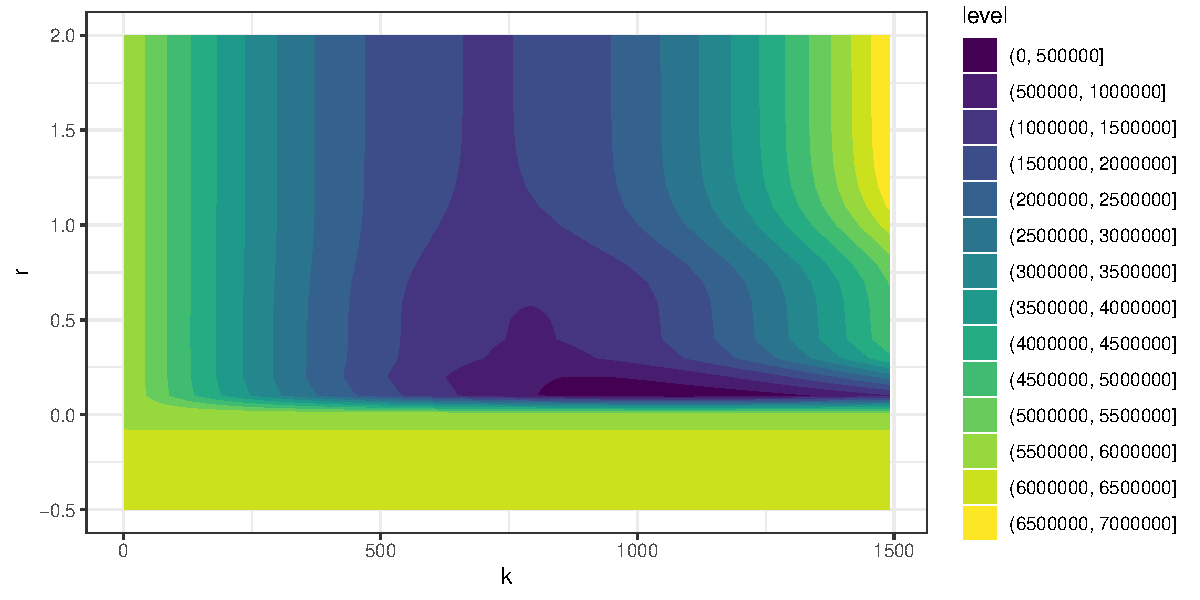
\includegraphics[width=16cm,height=8cm]{imgs/space.pdf}}
  \captionsetup{font=footnotesize,width=15cm}
  \caption{\small Curvas de nível de Q.}
\end{figure}

\newpage
\section{Algoritmo Newton-Raphson}

Usando o método iterativo de Newton-Raphson

\begin{align}
\hat{\bm{\theta}}_{k+1}=\hat{\bm{\theta}}_{k}-[\bf{H}(\hat{\bm{\theta}}_k)]^{-1}\nabla Q(\hat{\bm{\theta}}_k)
\end{align}

Onde $\bm{\theta}_k=[K_{k},r_{k}]$,Nota-se que o método não é eficiente quando o chute inicial de $r$ é ruim, por vezes caindo em mínimos locais ou por ventura dando erro por cair em uma divisão por zero numérico. Observa-se que um bom \textit{range} de valores iniciais para $r$ é (.07,.16). Optou-se então por testar o método para os seguintes pontos iniciais: $\theta^{(1)}_{0}=[900,0.1]$, $\theta^{(2)}_{0}=[500,0.1]$ , $\theta^{(3)}_{0}=[1024,0.15]$, $\theta^{(4)}_{0}=[2000,0.15]$ e $\theta^{(4)}_{0}=[1024,0.5]$. 

\begin{table}[H]
\centering
\caption{Resultados do método Newton-Raphson.}
\begin{tabular}{ccccc}
\hline
$\theta_{0}$      & $\hat{r}$ & $\hat{K}$ & iter & $Q(\hat{r},\hat{K})$ \\ \hline
$K_0=900,r=0.1$   & 0.11793   & 1033.5623 & 3    & 83240.55             \\
$K_0=500,r=0.1$   & 0.11795   & 1033.5153 & 5    & 83240.49             \\
$K_0=1024,r=0.15$ & 0.11795   & 1033.5156 & 3    & 83240.49             \\
$K_0=2000,r=0.15$ & 0.11795   & 1033.5164 & 4    & 83240.49             \\
$K_0=1024,r=0.5$ & 2.18865   & 709.2222 & 7    & 1477923             \\ \hline
\end{tabular}
\end{table}

Abaixo é plotado o gráfico de $N_t=f_{r,K}(t)$ com os valores estimados. Podemos observar um ajuste razoável.

\begin{figure}[H]
  \centering
  {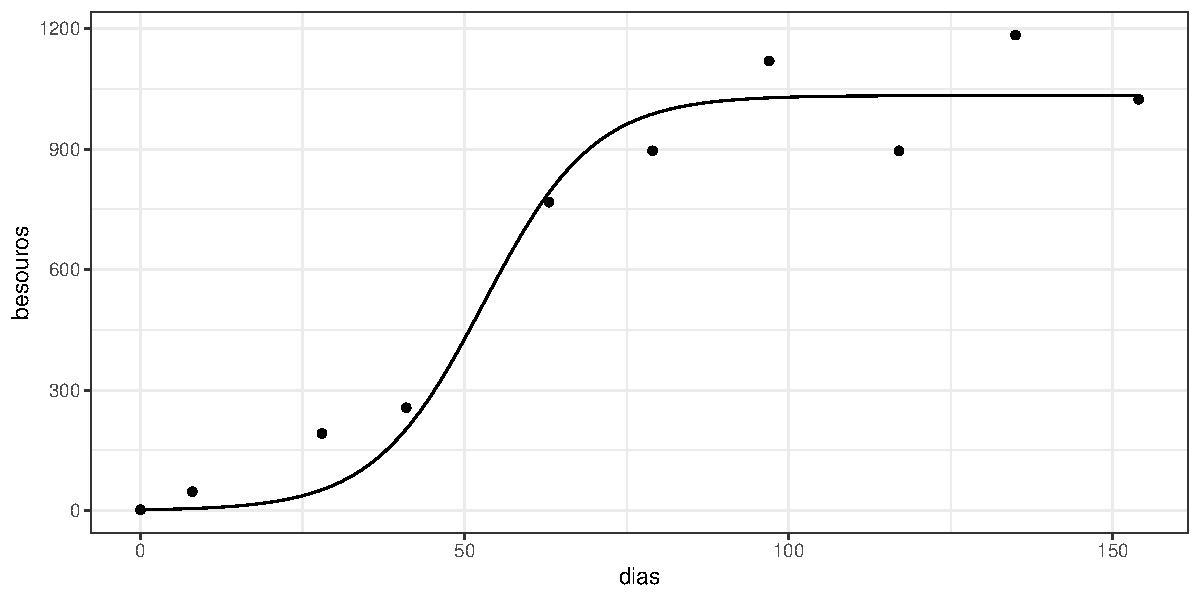
\includegraphics[width=16cm,height=8cm]{imgs/NR.pdf}}
  \captionsetup{font=footnotesize,width=15cm}
  \caption{\small Curva ajustada nos dados a partir do método de Newton-Raphson ($K=1033.56,r=0.11795$).}
\end{figure}


\newpage
\section{Algoritmo \textit{line-search}}
Para implementação do \textit{line-search}, devemos encontrar $\gamma_{k+1} (0,\infty)$ tal que $Q(\bm{\theta}_k - \gamma_k\bf{p}_{k})$ seja ótima em função de $\gamma$, em que $\bf{p}_{k}=[\bf{H}(\hat{\bm{\theta}}_k)]^{-1}\nabla Q(\hat{\bm{\theta}}_k)$

\begin{align*}
Q(\bm{\theta}_k - \gamma_k\bf{p}_{k})&=\sum_{i=1}^{m}\left(N_i - f_{\gamma,r,K}(t_i)\right)^2
\end{align*}
em que 
\begin{align*}
f_{\gamma,r,K}(t_i)=\frac{(K-\gamma \bf{p}_{1}) N_0}{N_0 + (K-\gamma \bf{p}_{1}-N_0)\exp{\{-(r-\gamma \bf{p}_{2})t\}}}
\end{align*}

Para tanto devemos obter o valor de $\gamma$ que zera a função abaixo.
\begin{align*}
\frac{\partial Q}{\partial \gamma}(\gamma,r,K)=\sum_{i=1}^{m}\left[(-2N_i\frac{\partial  f_{\gamma,r,K}}{\partial \gamma} + 2f_{\gamma,r,K}\frac{\partial  f_{\gamma,r,K}}{\partial \gamma} ) \right]
\end{align*}

Todavia observou-se que $\partial f_{\gamma,r,K}/\partial \gamma$ possui uma forma fechada bem complexa, impossibilitando uma solução analítica, portanto optou-se por utilizar método numéricos já implementados no R para computar $\gamma_{k}$, adicionalmente foi necessário restringir $\gamma>0.5$ pois sem essa restrição usualmente apontava um $\gamma_{k}\approx 0$ segundo as ressalvas citadas no método de Newton-Raphson.
\begin{table}[H]
\centering
\caption{Resultados do método line-search.}
\begin{tabular}{ccccc}
\hline
$\theta_{0}$      & $\hat{r}$ & $\hat{K}$ & iter & $Q(\hat{r},\hat{K})$ \\ \hline
$K_0=900,r=0.1$   & 0.11795   & 1033.5153 & 4    & 83240.55             \\
$K_0=500,r=0.1$   & 0.11795   & 1033.5152 & 4    & 83240.49             \\
$K_0=1024,r=0.15$ & 0.11795   & 1033.5156 & 3    & 83240.49             \\
$K_0=2000,r=0.15$ & 0.11795   & 1033.5164 & 3    & 83240.49             \\
$K_0=1024,r=0.5$ & 0.11795   & 1033.5153 & 28    & 1477923             \\ \hline
\end{tabular}
\end{table}
Com a implementação do \textit{line-search}, observou-se um ganho sob o número de interações em relação ao método anterior e adicionalmente os pontos iniciais que levaram a não convergência para o mínimo global dessa vez convergiram corretamente.

\begin{figure}[H]
  \centering
  {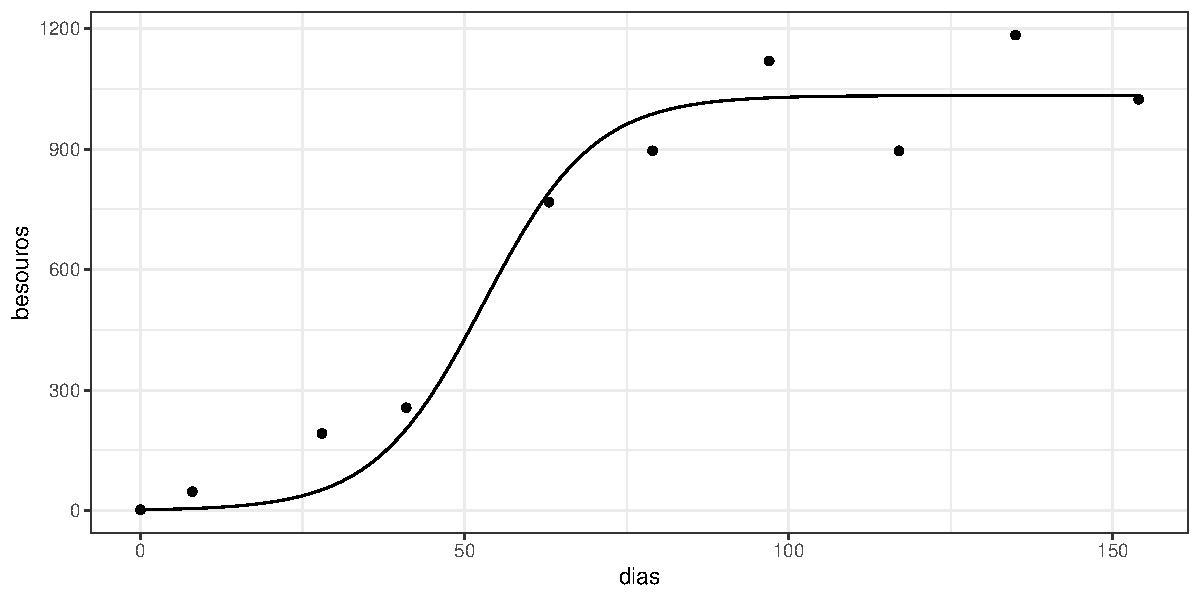
\includegraphics[width=16cm,height=8cm]{imgs/NR.pdf}}
  \captionsetup{font=footnotesize,width=15cm}
  \caption{\small Curva ajustada nos dados a partir do método de \textit{line-search} ($K=1033.56,r=0.11795$).}
\end{figure}
\section{Algoritmo Escore de fisher}
Assumindo $\log(N_t)\sim N(log\{f_{r,K}(t)\},\sigma^2)$, a verosimilhança é dada por 

\begin{align*}
L(\bm{\theta})=\prod_{i=1}^{m}\left[\frac{1}{\sqrt{2\pi\sigma^2}}\exp{\left(\frac{-1}{2\sigma^2}(\log(N_t)-\log(f_{r,K}))^2\right)}\right]
\end{align*}

Sendo $\theta=[r,K,\sigma^2]^{\top}$ , portanto a log-verosimilhança é dada por

\begin{align*}
\ell(\bm{\theta})=\sum_{i=1}^{m}\left[\frac{-1}{2}\log(2\pi\sigma^2)-\frac{1}{2\sigma^2}(\log(N_t)-\log(f_{r,K}))^2         \right]
\end{align*} 

\subsection*{Vetor gradiente e informação de fisher}
O vetor gradiente da função $\ell$ dos parâmetros r, K e $\sigma^2$ é dada por.
\begin{equation}
\nabla \ell(\bm{\theta})=\left[\frac{\partial \ell}{\partial K}(\bm{\theta}),\frac{\partial \ell}{\partial r}(\bm{\theta}),\frac{\partial \ell}{\partial \sigma^2}(\bm{\theta}) \right]
\end{equation}

em que

\begin{align*}
\frac{\partial \ell}{\partial r}(\bm{\theta})&=\frac{-1}{2\sigma^2}\sum_{i=1}^{m}\left[-2\log(N_t)\frac{\partial \log(f_{r,K})}{\partial r} + \frac{\partial \log^{2}(f_{r,K})}{\partial r} \right]\\\\
\frac{\partial \ell}{\partial K}(\bm{\theta})&=\frac{-1}{2\sigma^2}\sum_{i=1}^{m}\left[-2\log(N_t)\frac{\partial \log(f_{r,K})}{\partial K} + \frac{\partial \log^{2}(f_{r,K})}{\partial K} \right]\\\\
\frac{\partial \ell}{\partial \sigma^2}(\bm{\theta})&=\sum_{i=1}^{m}\left[\frac{-1}{2\sigma^2} + \frac{1}{2(\sigma^2)^2} (\log(N_t)-\log(f_{r,K}))^2 \right]
\end{align*}

Temos que as componentes do vetor gradiente depende de algumas derivadas parciais, que são apresentadas abaixo.

\begin{align*}
\frac{\partial \log(f_{r,K})}{\partial r}&=\frac{1}{f_{r,K}}\frac{\partial f_{r,K}}{\partial r}\\\\
\frac{\partial \log^{2}(f_{r,K})}{\partial r}&=2\log(f_{r,K})\frac{\partial \log(f_{r,K})}{\partial r}=2\log(f_{r,K})\frac{1}{f_{r,K}}\frac{\partial f_{r,K}}{\partial r}\\\\
\frac{\partial \log(f_{r,K})}{\partial K}&=\frac{1}{f_{r,K}}\frac{\partial f_{r,K}}{\partial K}\\\\
\frac{\partial \log^{2}(f_{r,K})}{\partial K}&=2\log(f_{r,K})\frac{\partial \log(f_{r,K})}{\partial K}=2\log(f_{r,K})\frac{1}{f_{r,K}}\frac{\partial f_{r,K}}{\partial K}
\end{align*}

Já a informação de fisher é dada pelo negativo da esperança da matriz hessiana de $\ell(\bm{\theta})$.

\begin{equation}
\mathcal{I}(\bm{\theta})=-\mathbb{E}[\bf{H_{\ell}(\bm{\theta})}]
\end{equation}

em que 

\begin{equation}
\bf{H}_{\ell}(\bm{\theta})=\begin{bmatrix}
\frac{\partial^2\ell }{\partial r^2}(\bf{\theta}) &\frac{\partial^2\ell }{\partial r\partial K}(\bf{\theta})  & \frac{\partial^2\ell }{\partial r\partial \sigma^2}(\bf{\theta}) \\ 
- & \frac{\partial^2\ell }{\partial K^2}(\bf{\theta}) &\frac{\partial^2\ell }{\partial K\partial \sigma^2}(\bf{\theta})  \\ 
- & - & \frac{\partial^2\ell }{\partial (\sigma^2)^2}(\bf{\theta})
\end{bmatrix}
\end{equation}
\newpage
\section*{Apêndice A}

\subsection*{A.1 Derivadas parciais no R}
\begin{lstlisting}[language=R]
ft <- function(param,data,N0){
  t <- data$dias
  k <- param[1]
  r <- param[2]
  output <- (k*N0) / (N0 + (k-N0)*exp(-r*t)) 
  return(output)
}
# Função Objetivo
Q <- function(param,data,N0){
  ti <- data[,1]
  Ni <- data[,2]
  frk <- ft(param,data,N0)
  output <- sum((Ni-frk)^2)
  return(output)
}
# Derivadas parciais de 1 e 2 ordem da função f
dfdr <- function(param,data,N0){
  t <- data$dias
  K <- param[1]
  r <- param[2]
  output <- (K*N0*( (K-N0)*exp(-r*t)*t ))/ ((N0 + (K-N0)*exp(-r*t))^2)
  return(output)
}

dfdK <- function(param,data,N0){
  t <- data$dias
  K <- param[1]
  r <- param[2]
  output <- (N0*(-exp(-r*t)*N0+N0)) / (N0+exp(-r*t)*(K-N0))^2
  return(output)
}

d2fdr2 <- function(param,data,N0){
  t <- data$dias
  K <- param[1]
  r <- param[2]
  output <- (K*exp(-2*r*t)*N0*(t^2)*(-exp(r*t)*N0-N0+K)*(K-N0))/  ((N0+exp(-r*t)*(K-N0))^3)
  return(output)
}

d2fdK2 <- function(param,data,N0){
  t <- data$dias
  K <- param[1]
  r <- param[2]
  output <- (2*exp(-r*t)*N0*(-exp(-r*t)*N0+N0))/((N0+exp(-r*t)*(K-N0))^3)
  return(output)
}

d2fdkdr <- function(param,data,N0){
  t <- data$dias
  K <- param[1]
  r <- param[2]
  output <- (exp(-r*t)*N0*N0*t*(exp(-r*t)*N0-N0+2*K-K*exp(-r*t)))/((N0+exp(-r*t)*(K-N0))^3)
  return(output)
}

# Veto gradriente da função objetivo
dQdr <- function(param,data,N0){
  K <- param[1]
  r <- param[2]
  df <- data%>%
    mutate(aux=ft(param = param,data=data,N0 = N0),
           dQdr=-2*besouros*dfdr(param = param,data=data,N0 = N0) +
             2*aux*dfdr(param = param,data=data,N0 = N0))
  output <- sum(df$dQdr)
  return(output)
}

dQdK <- function(param,data,N0){
  K <- param[1]
  r <- param[2]
  df <- data%>%
    mutate(aux=ft(param = param,data=data,N0 = N0),
           dQdk=-2*besouros*dfdK(param = param,data=data,N0 = N0) +
             2*aux*dfdK(param = param,data=data,N0 = N0))
  output <- sum(df$dQdk)
  return(output)
}

gradQ <- function(param,data,N0){
  K <- param[1]
  r <- param[2]
  gradR <- dQdr(param,data,N0)
  gradK <- dQdK(param,data,N0)
  gradiente <- c(gradK,gradR)
  return(gradiente)
}

# Matriz Hessiana da função objetivo
d2Qdr2 <- function(param,data,N0){
  K <- param[1]
  r <- param[2]
  df <- data%>%
    mutate(aux=ft(param = param,data=data,N0 = N0),
           d2Qdr2=-2*besouros*d2fdr2(param,data,N0)+2*dfdr(param,data,N0)^2 +
             2*ft(param,data,N0)*d2fdr2(param,data,N0))
  output <- sum(df$d2Qdr2)
  return(output)
}

d2Qdk2 <- function(param,data,N0){
  K <- param[1]
  r <- param[2]
  df <- data%>%
    mutate(aux=ft(param = param,data=data,N0 = N0),
           d2QdK2=-2*besouros*d2fdK2(param,data,N0)+2*dfdK(param,data,N0)^2 +
             2*ft(param,data,N0)*d2fdK2(param,data,N0))
  output <- sum(df$d2QdK2)
  return(output)
}

d2QdKdr <- function(param,data,N0){
  K <- param[1]
  r <- param[2]
  df <- data%>%
    mutate(aux=ft(param = param,data=data,N0 = N0),
           d2QdKdr=-2*besouros*d2fdkdr(param,data,N0)+
             2*dfdK(param,data,N0)*dfdr(param,data,N0)+
             2*ft(param,data,N0)*d2fdkdr(param,data,N0))
  output <- sum(df$d2QdKdr)
  return(output)
}

hessianQ <- function(param,data,N0){
  A11 <- d2Qdk2(param,data,N0)
  A22 <- d2Qdr2(param,data,N0)
  A12 <- A21 <- d2QdKdr(param,data,N0)
  hessiana <- matrix(data = c(A11,A21,A12,A22),2,2)
  return(hessiana)
}

\end{lstlisting}
\newpage
\subsection*{A.2 Newton-Raphson}
\begin{lstlisting}[language=R]
NR <- function(theta_k,data,N0,epsilon,criterium){
  iter=0
  while (criterium>epsilon) {
    iter <- iter + 1
    theta_k_plus_1 <- theta_k - solve(hessianQ(param=theta_k,data=data,N0=2))%*%gradQ(param=theta_k,data=data,N0=2)
    criterium <- abs(Q(param = theta_k_plus_1,data = data,N0=2)/Q(param = theta_k,data = data,N0=2) - 1)
    theta_k <- theta_k_plus_1
  }
  output <- list(iter=iter,theta=theta_k,Q_func=Q(param=theta_k,data,N0))
  return(output)
}
\end{lstlisting}
\subsection*{A.3 line search}
\begin{lstlisting}[language=R]
# Algorítimo de line search
ft_ls <- function(gama,param,data,N0){
  t <- data$dias
  k <- param[1]
  r <- param[2]
  p <- solve(hessianQ(param=param,data=data,N0=2))%*%gradQ(param=param,data=data,N0=2)
  pk <- p[1];pr=p[2]
  output <- ((k-gama*pk)*N0) / (N0 + (k-gama*pk-N0)*exp(-(r-gama*pr)*t)) 
  return(output)
}
Q_ls <- function(gama,param,data,N0){
  ti <- data$dias
  Ni <- data$besouros
  frk <- ft_ls(gama,param,data,N0)
  output <- sum((Ni-frk)^2)
  if(gama>.5){
    return(output)
  }else{
    return(Inf)
  }
}
ls <- function(theta_k,data,N0,epsilon,criterium){
  iter=0
  while (criterium>epsilon) {
    iter <- iter + 1
    gama <- optimize(f = Q_ls,interval = c(.5,2),param=theta_k,data=data,N0=N0)$minimum
    theta_k_plus_1 <- theta_k - gama*solve(hessianQ(param=theta_k,data=data,N0=2))%*%gradQ(param=theta_k,data=data,N0=2)
    criterium <- abs(Q(param = theta_k_plus_1,data = data,N0=2)/Q(param = theta_k,data = data,N0=2) - 1)
    theta_k <- theta_k_plus_1
  }
  output <- list(iter=iter,theta=theta_k,Q_func=Q(param=theta_k,data,N0))
  return(output)
}
\end{lstlisting}
\subsection*{A.4 Escore de fisher}
\begin{lstlisting}[language=R]
llk <- function(param,data,N0){
  K <- param[1]
  r <- param[2]
  sigma2 <- param[3]
  ti <- data[,1]
  Ni <- data[,2]
  frk <- ft(param,data,N0)
  output <- sum(-.5*log(2*pi*sigma2) -(1/(2*sigma2))*(log(Ni)-log(frk))^2 )
  if(sigma2>0 & r>0 & K>0){
    return(-output)
  }else{
    return(Inf)
  }
} 

dldK <- function(param,data,N0){
  K <- param[1]
  r <- param[2]
  sigma2 <- param[3]
  df <- data%>%
    mutate(aux=ft(param = param,data=data,N0 = N0),
           dfdK=dfdK(param,data,N0),
           dldK=(-1/(2*sigma2))* (-2*log(besouros)*(1/aux)*dfdK + 2*log(aux)*(1/aux)*dfdK ) )
  output <- sum(df$dldK)
  return(output)
}

dldr <- function(param,data,N0){
  K <- param[1]
  r <- param[2]
  sigma2 <- param[3]
  df <- data%>%
    mutate(aux=ft(param = param,data=data,N0 = N0),
           dfdr=dfdr(param,data,N0),
           dldr=(-1/(2*sigma2))* (-2*log(besouros)*(1/aux)*dfdr + 2*log(aux)*(1/aux)*dfdr ) )
  output <- sum(df$dldr)
  return(output)
}

dldsigma2 <- function(param,data,N0){
  K <- param[1]
  r <- param[2]
  sigma2 <- param[3]
  ti <- data[,1]
  Ni <- data[,2]
  frk <- ft(param,data,N0)
  output <- sum(-(1/(2*sigma2)) + (1/(2*sigma2^2))*(log(Ni)-log(frk))^2 )
  return(output)
}

gradllk <- function(param,data,N0){
  K <- param[1]
  r <- param[2]
  sigma2 <- param[3]
  gradR <- dldr(param,data,N0)
  gradK <- dldK(param,data,N0)
  gradsigma2 <- dldsigma2(param,data,N0)
  gradiente <- c(gradK,gradR,gradsigma2)
  return(gradiente)
}

Ed2ldr2 <- function(param,data,N0){
  K <- param[1]
  r <- param[2]
  sigma2 <- param[3]
  df <- data%>%
    mutate(aux=ft(param = param,data=data,N0 = N0),
           dfdr=dfdr(param,data,N0),
           d2fdr2=d2fdr2(param,data,N0),
           d2ldr2=(-1/(2*sigma2))* (-2*log(aux)*((1/aux)*d2fdr2-(aux^(-2))*(dfdr^2)) +
                  2*(((aux^(-2))*dfdr-(aux^(-2))*dfdr*log(aux))*dfdr + log(aux)*(1/aux)*d2fdr2)) )
  output <- sum(df$d2ldr2)
  return(output)
}

Ed2ldK2 <- function(param,data,N0){
  K <- param[1]
  r <- param[2]
  sigma2 <- param[3]
  df <- data%>%
    mutate(aux=ft(param = param,data=data,N0 = N0),
           dfdK=dfdK(param,data,N0),
           d2fdK2=d2fdK2(param,data,N0),
           d2ldK2=(-1/(2*sigma2))* (-2*log(aux)*((1/aux)*d2fdK2-(aux^(-2))*(dfdK^2)) +
                                      2*(((aux^(-2))*dfdK-(aux^(-2))*dfdK*log(aux))*dfdK + log(aux)*(1/aux)*d2fdK2)  ) )
  output <- sum(df$d2ldK2)
  return(output)
}

Ed2ldsigma22 <- function(param,data,N0){
  K <- param[1]
  r <- param[2]
  sigma2 <- param[3]
  ti <- data[,1]
  Ni <- data[,2]
  frk <- ft(param,data,N0)
  output <- sum((1/(2*sigma2^2)) - (1/(sigma2^3))*(sigma2))
  return(output)
}

Ed2ldKdr <- function(param,data,N0){
  K <- param[1]
  r <- param[2]
  sigma2 <- param[3]
  df <- data%>%
    mutate(aux=ft(param = param,data=data,N0 = N0),
           dfdK=dfdK(param,data,N0),
           dfdr=dfdr(param,data,N0),
           d2fdKdr=d2fdKdr(param,data,N0),
           d2ldKdr=(-1/(2*sigma2))* (-2*log(aux)*((1/aux)*d2fdKdr-(aux^(-2))*(dfdK*dfdr)) +
                                      2*(((aux^(-2))*dfdK-(aux^(-2))*dfdK*log(aux))*dfdK + log(aux)*(1/aux)*d2fdKdr)))
  output <- sum(df$d2ldKdr)
  return(output)
}

Ed2ldrdsigma2 <- function(param,data,N0){
  K <- param[1]
  r <- param[2]
  sigma2 <- param[3]
  df <- data%>%
    mutate(aux=ft(param = param,data=data,N0 = N0),
           dfdr=dfdr(param,data,N0),
           d2ldrdsigma2=(1/(2*sigma2^2))* (-2*log(aux)*(1/aux)*dfdr + 2*log(aux)*(1/aux)*dfdr ) )
  output <- sum(df$d2ldrdsigma2)
  return(output)
}

Ed2ldKdsigma2 <- function(param,data,N0){
  K <- param[1]
  r <- param[2]
  sigma2 <- param[3]
  df <- data%>%
    mutate(aux=ft(param = param,data=data,N0 = N0),
           dfdk=dfdr(param,data,N0),
           d2ldkdsigma2=(1/(2*sigma2^2))* (-2*log(aux)*(1/aux)*dfdk + 2*log(aux)*(1/aux)*dfdk))
  output <- sum(df$d2ldkdsigma2)
  return(output)
}

fisher_inf <- function(param,data,N0){
  A11 <- Ed2ldK2(param,data,N0)
  A22 <- Ed2ldr2(param,data,N0)
  A33 <- Ed2ldsigma22(param,data,N0)
  A12 <- A21 <- Ed2ldKdr(param,data,N0)
  A13 <- A31 <- Ed2ldKdsigma2(param,data,N0)
  A23 <- A32 <- Ed2ldrdsigma2(param,data,N0)
  FI <- matrix(c(A11,A21,A31,A12,A22,A32,A13,A23,A33),3,3)
  return(FI)
}

theta_k=c(1000,.1,1)
data=dados[-1,]
N0=2
EF <- function(theta_k,data,N0,epsilon,criterium){
  iter=0
  while (criterium>epsilon) {
    iter <- iter + 1
    theta_k_plus_1 <- theta_k + solve(-fisher_inf(param=theta_k,data=data,N0=2))%*%gradllk(param=theta_k,data=data,N0=2)
    criterium <- abs(llk(param = theta_k_plus_1,data = data,N0=2)/llk(param = theta_k,data = data,N0=2) - 1)
    theta_k <- theta_k_plus_1
  }
  output <- list(iter=iter,theta=theta_k,llk=llk(param=theta_k,data,N0))
  return(output)
}
\end{lstlisting}
\subsection*{A.4 Critério de parada}
O critério de parada adotado para as otimizações foi
\begin{equation}
|Q(K_{k+1},r_{k+1})/Q(K_{k},r_{k})-1|<\varepsilon=10^{-5}
\end{equation}

\section*{Apêndice B}

\end{document}
























